%\svnkwsave{$RepoFile: siminos/chao/exerFlow.tex $}
%\svnidlong {$HeadURL$}
%{$LastChangedDate$}
%{$LastChangedRevision$} {$LastChangedBy$}
%\svnid{$Id$}


\chapter{Exercises}
\label{sect:exerFlow}

\exercise{Birkhoff coordinates.}{\label{ex_birkhoff}
\index{Birkhoff!coordinates}
                                            \toCB
\PCedit{[Predrag 18apr2011 - not edited yet]}
In a plane billiard the ball travels between bounces
 along a straight line with a constant velocity--so the
4\dmn\ phase space flow can be reduced to a 2\dmn\ map
$\PoincM_{\Ssym{k} \leftarrow \Ssym{j}}$ that maps the
coordinates (Poincar\'e section $\PoincS_k$)
of the pinball from one disk edge to another.

A billiard flow has a natural Poincar\'e section
defined by Birkhoff coordinates $\arc_n$,
the arc length position of the $n$th bounce measured
along the billiard boundary,  % (\reffig{f-3disk}\,(b)),
and $\mompar_n= |p| \sin \phi_n$, the
momentum component parallel to the boundary, where $\phi_n$ is
the angle between the outgoing trajectory and the normal to the boundary.
We measure both the arc length $\arc$,
and the parallel momentum $\mompar$
counterclockwise relative to the outward normal%
. %(see \reffig{f-pinbAngles} as well as \reffig{FigIntroThreeA}).
In $\DOF=2$, the Poincar\'e section is a cylinder (topologically
an annulus),
% \reffig{f:BirkhoffCyl},
where the parallel momentum $\mompar$ ranges
for $-|p|$ to  $|p|$, and the $\arc$ coordinate is cyclic
along each connected component of $\partial Q$.
%\PC{label the two areas $Q_1$, $Q_2$ in \reffig{f:BirkhoffCyl}.
%Draw corresponding rectangles?}
The volume in the full phase space is preserved by the
Liouville theorem%
. % \refeq{LiuvVolCons}.
% The
Prove that the Birkhoff coordinates $x=(\arc,\mompar) \in \PoincS$,
% see \reffig{f-pinbAngles},
are the natural choice,
because with them the Poincar\'e return map
preserves the phase space volume of the $(\arc,\mompar)$ parameterized
Poincar\'e section
(a perfectly good coordinate set $(\arc, \phi)$ does not do that).
\index{Birkhoff!coordinates}
%\exerbox{ex_birkhoff}
% and they are easy to extract from the pinball trajectory.
% \toSect{c_buni_curv}

Without loss of generality we set $m=|v|=|p|=1$. % throughout.
Poincar\'e section condition eliminates one dimension, and the
energy conservation
$|p|=1$ eliminates
another, so the Poincar\'e section return map \PoincM\ is
$(2\DOF-2)$-dimensional.


Just after
the moment of impact the trajectory  is defined by $\arc_n$, the arc-length
position of the $n$th bounce along the billiard wall, and
$\mompar_n= p \sin \phi_n$
the momentum component parallel to the billiard wall
at the point of impact,
 reffig~{FigIntroThreeA}.

Prove that these coordinates (due to Birkhoff) are phase space volume
preserving.

The {\jacobianM} for the $n$th free flight segment is
\beq
\monodromy_{T}(x_n) = \MatrixII{1}{\timeSegm{n}}{0}{1}
\, .
\label{hor}
\eeq
The \jacobianM\ associated with the reflection is
\beq
\monodromy_R(x_n) = - \MatrixII{1}    {0}
                { r_n }{1}
\,, \quad \quad
r_n = {2 \over \curvR_n \cos\phi_n }
\, .
\label{hur}
\eeq
The full \jacobianM\ for $\cl{p}$ consecutive bounces describes a beam of
trajectories defocused  by $\monodromy_T$ along the free flight (the
$\timeSegm{n}$ terms below) and defocused/refocused at reflections by
$\monodromy_R$ (the $r_n$ terms below)
\beq
\monodromy_p = (-1)^{\cl{p}} \prod_{n={\cl{p}}}^{1}
          \MatrixII{1}{  \timeSegm{n} }
                   {0}  {1}
          \MatrixII{1}{0}
                   { r_{n}}{1}
\, ,
\ee{eq_her}
where $\timeSegm{n}$ is the flight time of the $k$th free-flight segment
of the orbit, $r_n = {2 / \curvR_n \cos\phi_n }$ is the defocusing due to
the $k$th  reflection, and $ \curvR_n$ is the  radius of curvature of the
billiard boundary at the  $n$th scattering point

Verify the ChaosBook formulas \refeq{hor}, \refeq{eq_her} and
\refeq{eq_her}. Hint: is is more elegant if you derive them separately,
rather than going directly for the \refeq{eq_her} multiplied out.

No need to reinvent the wheel;
use the same notation as ChaosBook, \ie, $\arc_i$ instead
$a_i \theta$.
} %end \exercise{Birkhoff coordinates.}


\solution{ex_birkhoff}{Birkhoff coordinates.}{
%
%%%%%%%%%%%%%%%%%%%%%%%%%%%%%%%%%%%%%%%%%%%%%%%%%%%%%%%%%%%%%%%%%%
\BFIG{0.90}{exr2-1} %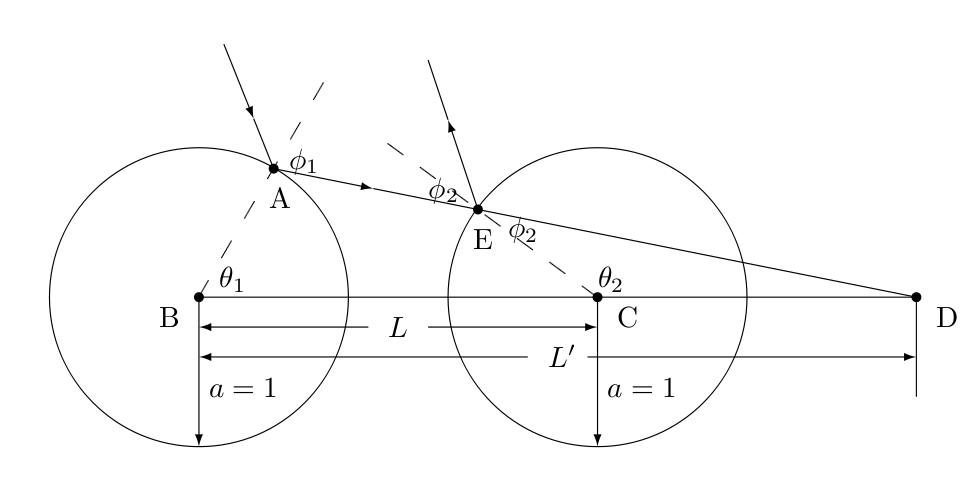
\includegraphics[width=0.40\textwidth]{exr2-1}}
{}{
Poincar\'e section coordinates for the 3-disk game of pinball.
    }{Fig:exr2-1}
%%%%%%%%%%%%%%%%%%%%%%%%%%%%%%%%%%%%%%%%%%%%%%%%%%%%%%%%%%%%%%%%%
%
Assume the radius of two circles is $a=1$, the distance between the
centers of two circles is $L$, the magnitude of the ball's momentum is 1.
Thus, $p\sin{\phi} = \sin{\phi}$. If we assume radius 1, the arclength
is numerically equal to the angle $\theta$ in the picture. Here we use
the arclength $\arc$, which is equal to $a_i \theta$.

First, we have to find the
map:$(\arc_{1},\sin(\phi_{1}))\mapsto(\arc_{2},\sin(\phi_{2}))$. Look at
${\Delta}ABD$, by Sine Theorem, we have
$\frac{\sin({\pi}-\phi_{i})}{\overline{BD}} =
\frac{\sin(\beta)}{\overline{AB}}$, where $\overline{BD} = L^{'}$,
$\overline{AB} = a$, $\sin(\pi-\phi_{1}) = \sin(\phi_{1})$
\[
\Rightarrow \frac{\sin(\phi_{1})}{L^{'}} = \frac{\sin(\beta)}{R}
\]
Look at ${\Delta}ECD$, still by Sine Theorem, we have
$\frac{\sin(\beta)}{\overline{EC}} =
\frac{\sin(\phi_{2})}{\overline{CD}}$, where $\overline{EC} = a$,
$\overline{CD} = L^{'}-L$
\bea
\Rightarrow \frac{\sin(\phi_{2})}{L_{'}-L} &=& \frac{\sin(\beta)}{a}
\continue
\beta &=& \phi_{1}-\frac{\arc_{1}}{a}
\nnu
\eea
From the first equation, we have
\[
L_{'} = \frac{\sin(\phi_{1})}{\sin(\beta)}a = \frac{\sin(\phi_{1})}{\sin(\phi_{1}-\arc_{1})}
\]
Substitute this into the second equation, we have
\beq\displaystyle\frac{\sin(\phi_{2})}{\frac{\sin(\phi_{1})}{\sin(\phi_{1}-\frac{\arc_{1}}{a})}a-L}
= \frac{\sin(\phi_{1}-\frac{\arc_{1}}{a})}{a}\eeq
\beq\Rightarrow \sin(\phi_{2}) = \sin(\phi_{1})-\frac{L}{a}\sin(\phi_{1}-\frac{\arc_{1}}{a}) \eeq
Also we have
\(
\frac{\arc_{2}}{a} = \pi-\phi_{2}-\beta = \pi-\phi_{2}-(\phi_{1}-\frac{\arc_{1}}{a})
\,.
\)
Now we have the map. Next step is to show that it is phase-space volume preserving.

Rewrite the map by substituting $p_{i} = \sin(\phi_{i}),\phi_{i} = \arcsin(p_{i})$:
\beq p_{2} = p_{1}-\frac{L}{a}p_{1}\cos(\frac{\arc_{1}}{a})+\frac{L}{a}\sqrt{1-p_{1}^{2}}\sin(\frac{\arc_{1}}{a}) \eeq
\beq \frac{\arc_{2}}{a} = \pi+\frac{\arc_{1}}{a}-\arcsin(p_{1})-\arcsin(p_{2}) \eeq

\begin{eqnarray}
dp_{2}&=&dp_{1}-\frac{L}{R}\cos(\frac{\arc_{1}}{a})dp_{1}+\frac{L}{a}\sin(\frac{\arc_{1}}{a})p_{1}d\frac{\arc_{1}}{a}-
\frac{Lp_{1}\sin(\frac{\arc_{1}}{a})}{a\sqrt{1-p_{1}^{2}}}dp_{1}+
\\\nonumber&&\frac{L}{a}\sqrt{1-p_{1}^{2}}\cos{\frac{\arc_{1}}{a}}d\frac{\arc_{1}}{a}\\\nonumber
&=&(1-\frac{L}{a}\cos{\frac{\arc_{1}}{a}}-\frac{Lp_{1}\sin(\frac{\arc_{1}}{a})}{a\sqrt{1-p_{1}^{2}}})dp_{1}
+(\frac{L}{a}\sin(\frac{\arc_{1}}{a})p_{1}+\frac{L}{a}\sqrt{1-p_{1}^{2}}\cos{\frac{\arc_{1}}{a}})d\frac{\arc_{1}}{a}\\\nonumber
d\frac{\arc_{2}}{a}&=&d\frac{\arc_{1}}{a}-\frac{1}{\sqrt{1-p_{1}^{2}}}dp_{1}-\frac{1}{\sqrt{1-p_{2}^{2}}}dp_{2}\\\nonumber
dp_{2}\wedge d\frac{\arc_{2}}{a}&=& (1-\frac{L}{a}\cos(\frac{\arc_{1}}{a})-\frac{Lp_{1}\sin(\frac{\arc_{1}}{a})}{a\sqrt{1-p_{1}^{2}}})dp_{1}{\wedge}d\frac{\arc_{1}}{a}+\\&&\frac{1}{\sqrt{1-p_{1}^{2}}}(\frac{L}{a}\sin(\frac{\arc_{1}}{a})p_{1}
+\frac{L}{a}\sqrt{1-p_{1}^{2}\cos(\theta_{1})})dp_{1}\wedge d\frac{\arc_{1}}{a}\\\nonumber
&=&dp_{1}\wedge d\frac{\arc_{1}}{a}\\
&&\Rightarrow dp_{2}\wedge d\arc_{2} = dp_{1}\wedge d\arc_{1}
\end{eqnarray}
Now let's look at map for $\frac{s}{a}$. We can rewrite it as:
\[
 \frac{\arc_{2}}{a} - \frac{\arc_{1}}{a} = \pi-\arcsin(p_{1})-\arcsin(p_{2})
 \]
On the left hand side, $\frac{\arc_{2}}{a} - \frac{\arc_{1}}{a} =
\theta_{2}-\theta_{1}$ is independent of the choice of coordinate. Any
choice of start line of angle $\theta$ just varies up to a constant for
both $\theta_{2}$ and $\theta_{1}$, so won't affect the validity of the
demonstration.

If we take the radii unequal, $a_{1} \neq a_{2}$ we obtain the formula
for any smooth billiard, with $a_{i}$ being the local radius of curvature
at the $i$th bounce. now the absolute disk angles and the arc-length
parametrization are given by $\theta_{1}=\frac{\arc_1}{a_1}$,
$\theta_{2}=\frac{\arc_2}{a_2}$. Follow the same route above to obtain the
map:
\bea
p_{2} &=& \frac{a_1}{a_2}p_{1}-\frac{L}{a_2}p_{1}\cos(\frac{\arc_1}{a_1})+\frac{L}{a_2}\sqrt{1-p_1^2}\sin(\frac{\arc_1}{a_1})\\
\arc_{2} &=& \frac{a_2}{a_1}\arc_{1}+{\pi}a_{2}-a_{2}\arcsin(p_1)-a_{2}\arcsin(p_2)
\eea
By writing out the full derivative of $dp_2$ and $d\arc_2$ in terms of
$dp_1$ and $d\arc_1$, we can obtain the \JacobianM
\[
\left(
\begin{array}{c}
dp_2\\
d\arc_2
\end{array}
\right)
=
\left(
\begin{array}{cc}
\frac{dp_2}{dp_1} & \frac{dp_2}{d\arc_1}\\
\frac{d\arc_2}{dp_1} & \frac{d\arc_2}{d\arc_1}
\end{array}
\right)
\left(
\begin{array}{c}
dp_1\\
d\arc_1
\end{array}
\right)
\]
where
\bea
\frac{dp_2}{dp_1}&=&
\frac{a_1}{a_2}-\frac{L}{a_2}\cos(\frac{\arc_1}{a_1})-\frac{Lp_1}{a_2\sqrt{1-p_1^2}}\sin(\frac{\arc_1}{a_1})\\
\frac{dp_2}{d\arc_1}&=&
\frac{L}{a_{1}a_{2}}(p_1\sin(\frac{\arc_1}{a_1})+\sqrt{1-p_1^2}\cos(\frac{\arc_1}{a_1}))\\
\frac{d\arc_2}{dp_1}&=&
-\frac{a_2}{\sqrt{1-p_1^2}}-\frac{a_2}{\sqrt{1-p_2^2}}
(\frac{a_1}{a_2}-\frac{L}{a_2}\cos(\frac{\arc_1}{a_1})-\frac{Lp_1}{a_2\sqrt{1-p_1^2}}\sin(\frac{\arc_1}{a_1}))\\
\frac{d\arc_2}{d\arc_1}&=&
\frac{a_2}{a_1}-\frac{a_2}{\sqrt{1-p_2^2}}
\frac{L}{a_{1}a_{2}}(p_1\sin(\frac{\arc_1}{a_1})+\sqrt{1-p_1^2}\cos(\frac{\arc_1}{a_1}))
\eea
This yields $|J|=1$, Deities have been kind to me this time.
    }%end  \solution{ex_birkhoff}{Birkhoff coordinates.

\begin{description}\label{VarKSe}

\item[2011-09-26 ES to Chao] Derive the relation of $\nu$ to the parameter
$L$ used in \refref{SCD07}. What $L$ did Christiansen \etal\rf{Christiansen97}
study?

\item[2011-09-29]                                               \toCB
The equation used in \refref{SCD07}:
\beq
\mu_t = -\frac{1}{2}(\mu^2)_x - \mu_{xx} - \mu_{xxxx}, x \in [0,L]
\eeq
The equation used in \etal\rf{Christiansen97}
\beq
\mu'_{t'} = (\mu'^2)_{x'} - \mu'_{x'x'} - \nu\mu'_{x'x'x'x'}, x' \in [0,2\pi]
\eeq

Substitute the function and variables in the first equation with $t=\alpha t', x=\beta x', \mu=\gamma \mu'$,
we obtain
\beq
\frac{1}{\alpha}\mu'_{t'} = -\frac{1}{2}\frac{\gamma}{\beta}(\mu'^2)_{x'}-\frac{1}{\beta^2}\mu'_{x'x'}-\frac{1}{\beta^4}\mu'_{x'x'x'x'}, x' \in [0,\frac{L}{\beta}]
\eeq
Comparing with the second equation ,if we set
\beq
-\frac{1}{2}\frac{\alpha\gamma}{\beta} = \frac{\alpha}{\beta^2} = 1,
  \frac{\alpha}{\beta^4} = \nu,   \frac{L}{\beta} = 2\pi
\eeq, we will reach the second equation. Solving these equations, we obtain the relation
\beq L=\frac{2\pi}{\sqrt{\nu}}\eeq
In \rf{Christiansen97}, $\nu = 0.029910$ and $0.029924$, which corresponds to $L = 36.3305$ and $36.3220$

\end{description}
